% This is samplepaper.tex, a sample chapter demonstrating the
% LLNCS macro package for Springer Computer Science proceedings;
% Version 2.20 of 2017/10/04
%
\documentclass[runningheads]{llncs}
%
\usepackage{color}
\usepackage{graphicx}
\usepackage{subfigure}
\usepackage{braket}
\usepackage[final]{fixme}
\usepackage{amsmath,amsfonts,amssymb}
\usepackage{algorithm}
\usepackage[noend]{algpseudocode}
\usepackage{appendix}

\newcommand{\pp}[2]{\frac{\partial #1}{\partial #2}}
\newcommand{\dede}[2]{\frac{\delta #1}{\delta #2}}
\newcommand{\dd}[2]{\frac{\diff#1}{\diff#2}}
\newcommand{\half}{\frac 12}

\newcommand{\norm}[2]{\| #1 \|_{ #2 }}
\newcommand{\vnorm}[1]{\norm{ #1 }{V}}
\newcommand{\hnorm}[1]{\norm{ #1 }{H}}
\newcommand{\ltwonorm}[1]{\norm{ #1 }{2}}
\newcommand{\diff}[1]{\text{d} #1}

\newcommand{\Q}{\mathbf{q}}
\newcommand{\U}{\mathbf{u}}
\newcommand{\Z}{\mathbf{z}}
\newcommand{\V}{\mathbf{v}}
\newcommand{\Rd}{\mathbb{R}^{d}}
\newcommand{\RdM}{\mathbb{R}^{d\times M}}
\newcommand{\RdK}{\mathbb{R}^{d\times K}}
\newcommand{\nuinf}{\nu_\text{inf}}
\newcommand{\mdiv}{\text{div}}

\newtheorem{assumption}{Assumption}

% Used for displaying a sample figure. If possible, figure files should
% be included in EPS format.
%
% If you use the hyperref package, please uncomment the following line
% to display URLs in blue roman font according to Springer's eBook style:
% \renewcommand\UrlFont{\color{blue}\rmfamily}

\begin{document}
%
\title{Selective metamorphosis for growth modelling with applications to landmarks}
%
%\titlerunning{Abbreviated paper title}
% If the paper title is too long for the running head, you can set
% an abbreviated paper title here
%
\author{Andreas Bock\inst{1} \and  Alexis Arnaudon\inst{1} \and Colin Cotter\inst{1}}
%
\authorrunning{Bock et al.}
% First names are abbreviated in the running head.
% If there are more than two authors, 'et al.' is used.
%
\institute{Imperial College London}
%\email{lncs@springer.com}\\
%\url{http://www.springer.com/gp/computer-science/lncs} \and
%ABC Institute, Rupert-Karls-University Heidelberg, Heidelberg, Germany\\
%\email{\{abc,lncs\}@uni-heidelberg.de}}
%
\maketitle              % typeset the header of the contribution

\begin{abstract}
We present a framework for shape matching allowing users control of the degree
to which the matching is diffeomorphic in computational anatomy. This control is
given as a function defined over the image and parametrises the template
deformation. By modelling localised template deformation we have a mathematical
description of growth only in specified parts of an image. The location can
either be specified from prior knowledge of the growth location or learned from
data. For simplicity we consider landmark matching and infer the distribution of
a finite dimensional parametrisation of the control via Markov chain Carlo.
Preliminary numerical results are shown and future paths of investigation are
laid out. Well-posedness of this new problem is also shown together with an
analysis of the associated geodesic equations. 

\keywords{LDDMM \and MCMC \and Metamorphosis.}
\end{abstract}

\section{Introduction}

In computational anatomy
\cite{grenander1994representations,grenander1998computational}, one of the most
fundamental problem is to continuously deform an image or shape into another and
thereby obtain a natural notion of distance between them as the energy required
for this deformation.  These distances can then be used for image registration,
atlas construction, etc\dots see \cite{todo} for more applications. One of the
most common method to compute image deformations is based on diffeomorphic
deformations which assume that the images are continuously deformed into one
another with the additional property that the inverse deformation is also
continuous.  This is a strong requirement for images which implies that the
'mass' of any part of the image is conserved: we cannot create or close 'holes'.
This property is also a crucial property of fluid mechanics and in fact the
theory of diffeomorphic matching carrying the moniker \emph{Large Deformation
Diffeomorphic Metric Mapping} \cite{trouve1998diffeomorphisms,beg2005computing}
(LDDMM) has been inspired by fluid mechanics. Indeed, one of the central pillars
on which this field relies is the observation made by Arnold
\cite{arnold1966geometrie} that the geodesic equations for the diffeomorphism
group induced by divergence-free vector fields corresponded to that of
incompressible flows. See also ({\color{red} Refs of Darryl,
etc\dots.}{\color{green} Not too sure which fluids papers to reference here!}) 

If a strictly diffeomorphic matching is not possible or necessary, an extension
of LDDMM called metamorphosis \cite{trouve2005metamorphoses,holm2009euler} is
available which introduces a parameter $\sigma^2$ parametrizing the deviation
from diffeomorphic matching allowing for topological variations e.g. growth via
image intensity. In particular, if $\sigma^2=0$ the deformation is purely
diffeomorphic as in LDDMM. See
\cite{trouve1995infinite,trouve2005local,miller2001group} for technical details
pertaining to constructing the metamorphosis problem. x While diffeomorphic
paths always exists for landmark problems \cite{guo2006diffeomorphic} this
theory allows one to match images of shapes with different topological features,
which is ill-conditioned for standard LDDMM. Indeed, even inexact matching in
LDDMM for such problems yields large energies and spurious geodesics that do not
contribute to an intuitive macthing, see figure \ref{fig:mm_lddmm}. As observed
here, introducing $\sigma^2>0$ regularises the problem and qualitative improves
the matching.\\

In this work we modify metamorphosis to include a spatially dependent control
parameter $\nu(x)$ in order to selectively allow non-diffeomorphic
(\emph{metamorphic}) matching in parts of the image. For $\nu(x) = \sigma^2$ our
theory recovers the standard metamorphosis model. However, with a localised
$\nu(x)$ (e.g. Gaussian), we can selectively introduce metamorphosis in an image
and model local topological effects such as growth phenomena. The difficulty of
this problem is to infer the function $x\mapsto\nu(x)$ without prior knowledge
of the location of the topological effects. We will use a Markov chain Monte
Carlo (MCMC) approach to infer appropriate functions $\nu(x)$, such that the
topological effects are well described and a large part of the matching remains
diffeomorphic. For this paper, we will focus on landmark matching, but the
theory of selective metamorphosis can be extended to any data structures that
the classical metamorphosis or LDDMM theory can handle
\cite{bockarnaudoncotter2019}.

\begin{figure}
\centering
\begin{minipage}{\textwidth}
  \centering
    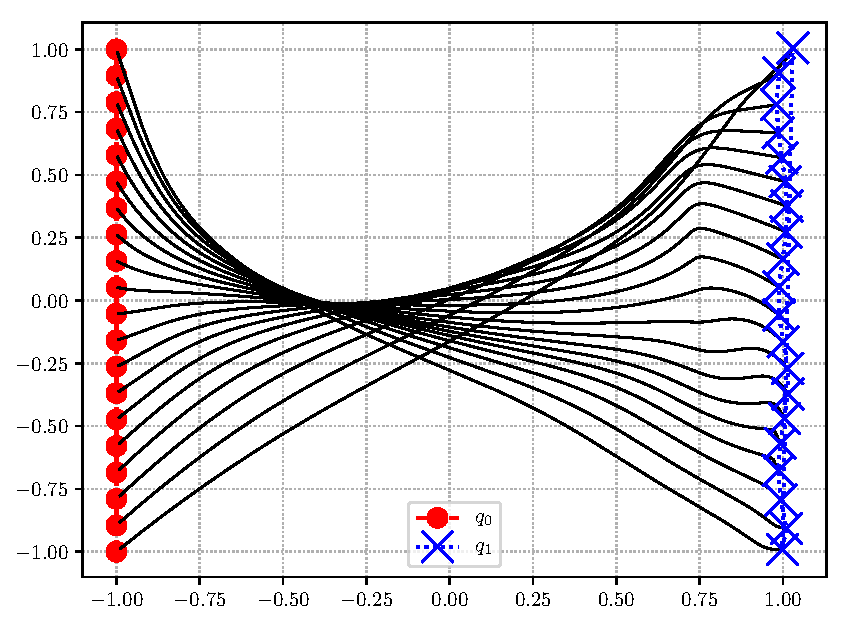
\includegraphics[width=.3\textwidth]{lddmm_criss_cross.pdf}\quad
    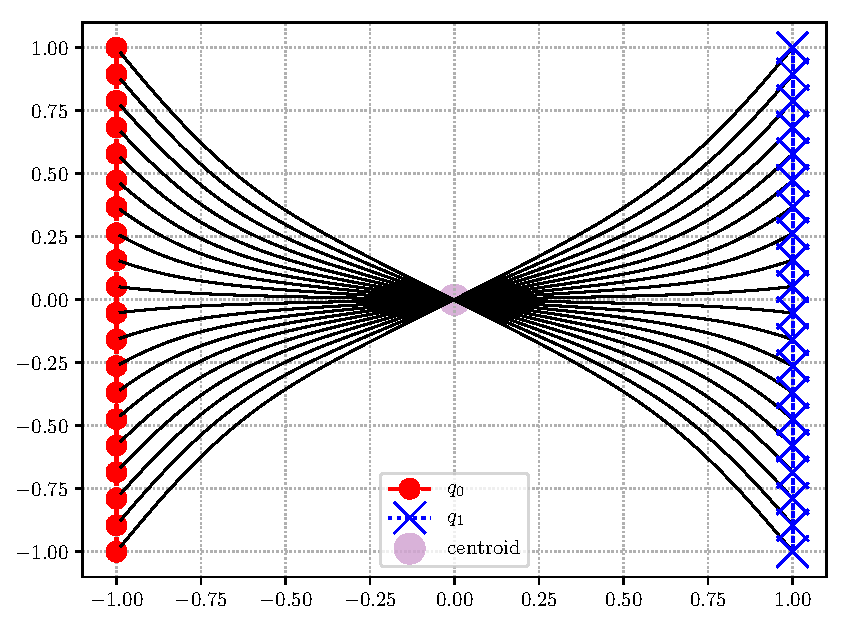
\includegraphics[width=.3\textwidth]{custom_nu_criss_cross.pdf}\quad
    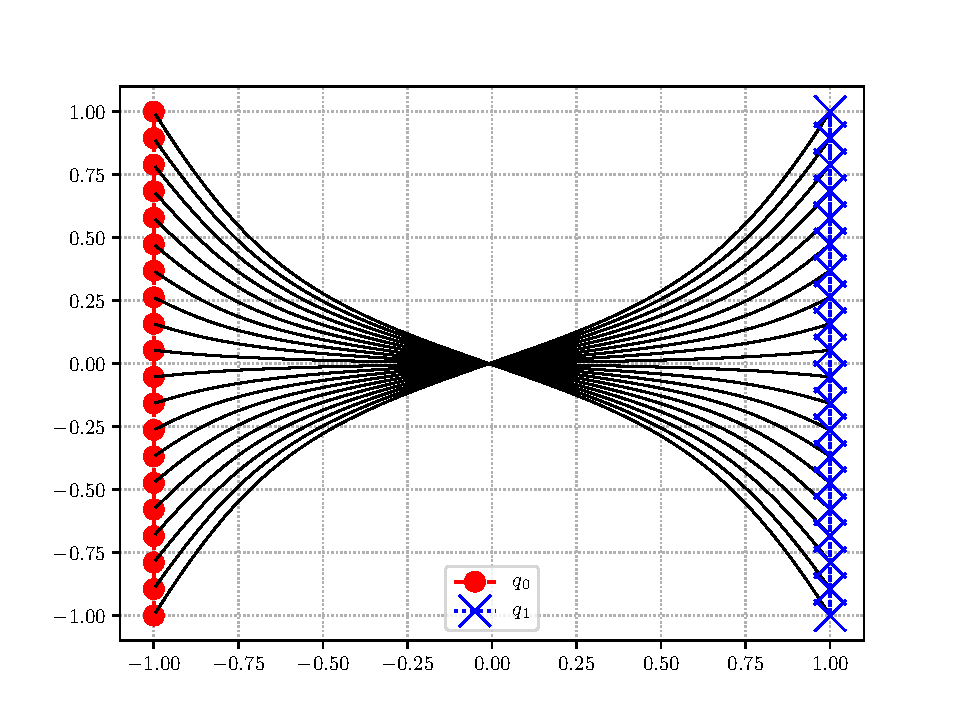
\includegraphics[width=.3\textwidth]{mm_criss_cross.pdf}\quad\\[0.25cm]
    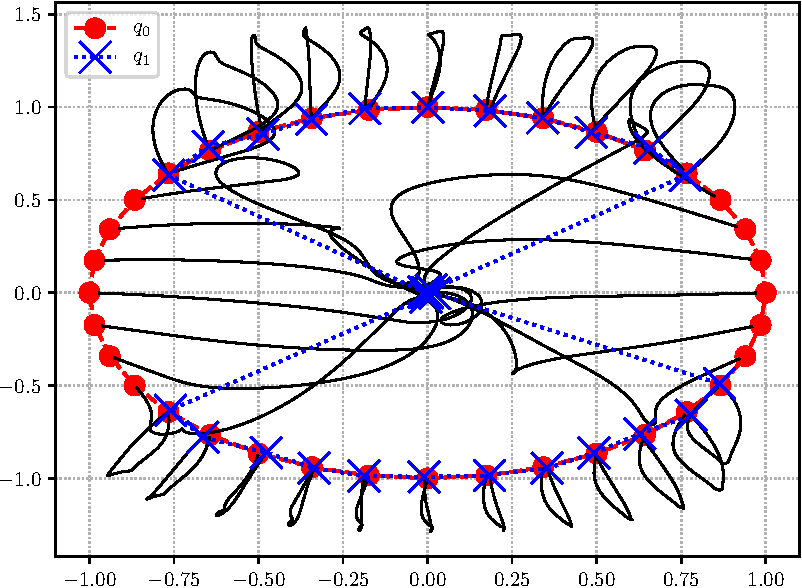
\includegraphics[width=.3\textwidth]{lddmm_squeeze.pdf}\quad
    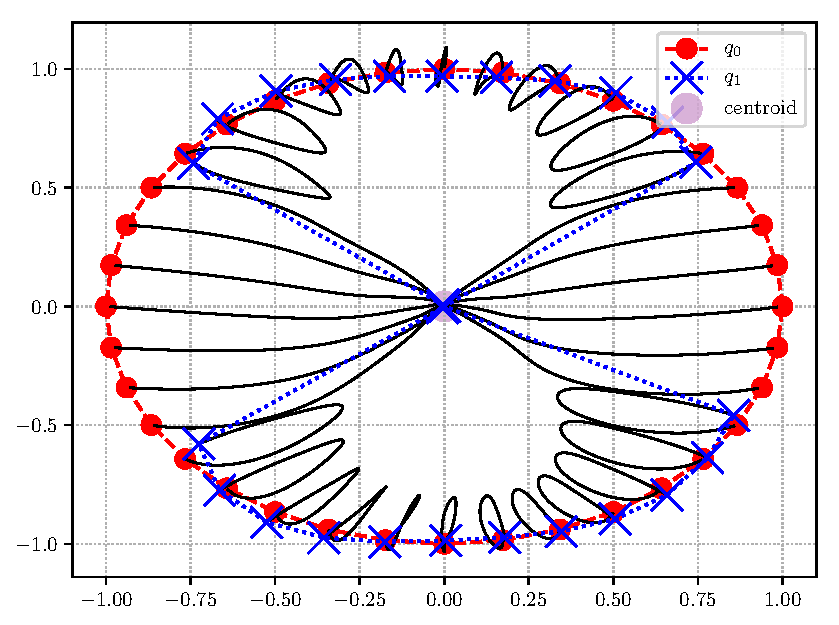
\includegraphics[width=.3\textwidth]{custom_nu_squeeze.pdf}\quad
    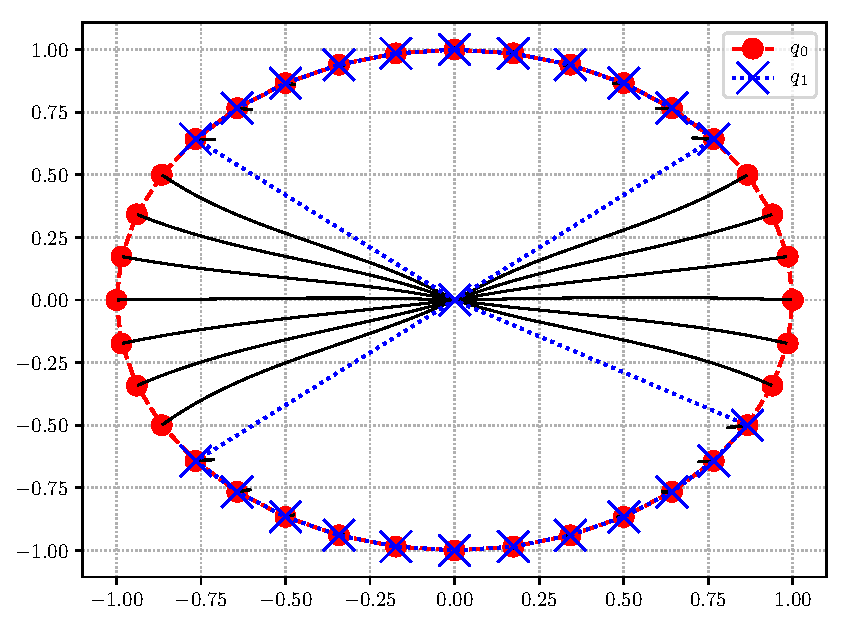
\includegraphics[width=.3\textwidth]{mm_squeeze.pdf}\quad
    %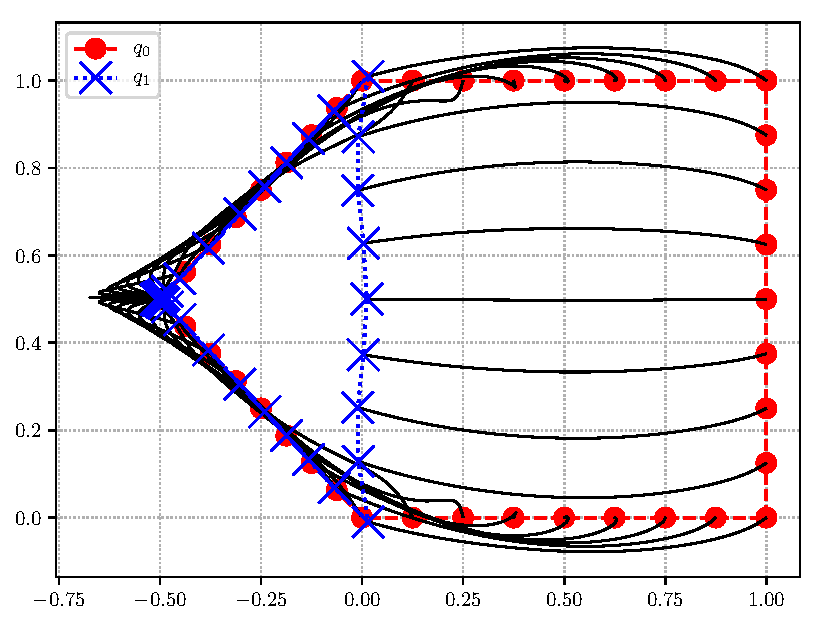
\includegraphics[width=.291\textwidth]{lddmm_pent_to_tri.pdf}\\[0.25cm]
    %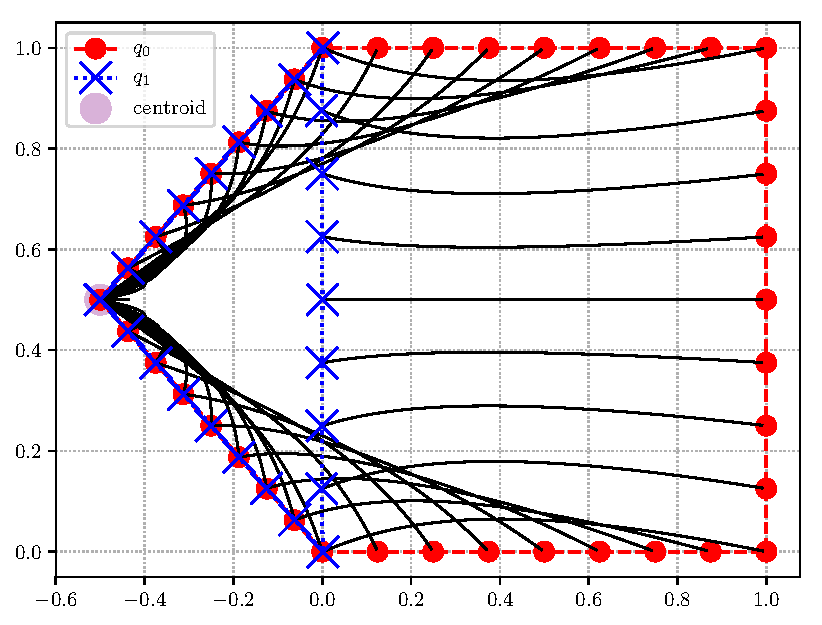
\includegraphics[width=.291\textwidth]{custom_nu_pent_to_tri.pdf}\\[0.25cm]
    %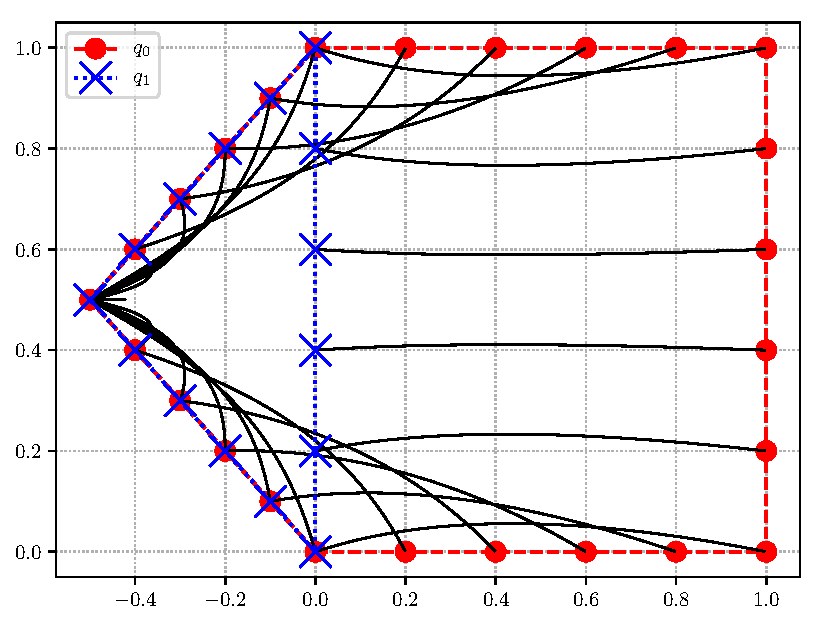
\includegraphics[width=.291\textwidth]{mm_pent_to_tri.pdf}
    \caption{{\color{red} Caption to be updated!}This figures illustrates landmark matching with classical LDDMM
    (top row), metamorphosis (bottom row) and selective metamorphosis (middle
    row).  We chose difficult matching for LDDMM, and we observe unrealistic
    landmark trajectories, with large resulting energies, or distances, whereas
    the metamorphosis  matching results in a more realistic landmark
    trajectories.  The selective metamorphosis has the extra advantage of only
    breaking the diffeomorphic property where needed in along the matching, thus
    preserving more of the desired diffeomorphic property of the matching.
    {\color{red} Add the middle row with position of $\nu$ fields as crosses,
    and value of the energy functional for each (larger for top and middle
    row)}}
    \label{fig:mm_lddmm}
\end{minipage}
\end{figure}

%In this paper we consider a generalisation of the classical metamorphosis
%problem. The purpose of this work is to allow singular control where
%metamorphosis occurs in space to allow practitioners in e.g. medical imaging to
%qualitatively assess different growth patterns. Owing to this observation we
%build a stochastic model on spatial domain and use develop an MCMC algorithm in
%order to infer where in space growth is the most likely.\\

{\bf Structure} This paper is organised as follows. We review the theory of
classical metamorphosis in section \ref{sec:bg} and extend it to selective
metamorphosis in \ref{sec:select_mm}.  We then introduce a Bayesian framework
for inferring the local metamorphosis parameter $\nu(x)$ in section
\ref{sec:bayesian} and apply this theory to a few landmark examples in section
\ref{sec:numerical}.

\section{Metamorphosis for Landmarks}\label{sec:bg}

In this paper we are concerned with diffeomorphometric approaches to image and
shape matching. One of the pillars on which this field relies is the observation
made by Arnold \cite{arnold1966geometrie} that, under certain conditions, a
time-dependent velocity field $u$ e.g. occupying some Hilbert space $u_t \in V$,
where $V$ is continuously embedded in $\textsf{C}_0^k(\Rd)$, $k\geq 1$ induces a
curve $\varphi_t$ on a subgroup $\text{Diff}_V$ of diffeomorphisms
\cite{younes2010shapes} via the following ordinary differential equation
\begin{align}
& \dot{\varphi_t} = u_t \circ \varphi_t\, , \qquad  \varphi_0 = \text{id}
  \label{diffeo}
\end{align}
This is often used in a minmisation problem where the objective is to match two
images $I_0$ and $I_1$:
\begin{align}
  E(u) = \int_0^1 \half\vnorm{u_t}^2 \diff{t} + \frac{1}{\sigma^2}
  S(I_0\circ\varphi_1, I_1)\longrightarrow \text{min}\, , \label{E-def}
\end{align}
where $S$ denotes a similarity measure between the deformed initial image
$I_0\circ \varphi_1$ and the target image $I_1$ to allow inexact matching
parametrised by $\sigma^2$. The LDDMM approach takes $S$ as an $L^2$ norm on
the difference between its arguments.\\

In order to simplify the exposition, we will consider singular solutions of this
problem, which are given by
\begin{align}
  \frac{\delta l}{\delta u} = \mathbf m(x) = \sum_{i=1}^M p_t^i \delta(x-q_t^i)\,, 
\end{align}
for $N$ landmarks with position $q_t^i\in \mathbb R^2 $ and momenta $p_t^i \in
\mathbb R^2$. The vector field is thus 
\begin{align}
  u(x) = \sum_{i=1}^M p_t^i K(x-q_t^i)\,, 
  \label{u-def}
\end{align}
where $K:\mathbb R^2\times \mathbb R^2\to \mathbb R$ is the kernel associated to
the norm $\|\cdot \|_V$.  For metamorphosis, we introduce a discrete template
variable $\boldsymbol \eta_t$ such that the deformation of a set of landmarks is
written as the composition of the template position and deformation as
\begin{align}
  \mathbf q_t = \varphi_t \boldsymbol \eta_t\, . 
  \label{q_t}
\end{align}
Then, we can define the template velocity as 
\begin{align}
  \mathbf z = \varphi_t \dot {\boldsymbol \eta}
  \label{z_eta}
\end{align}
and extend the energy \eqref{E-def} to 
\begin{align}
  \begin{split}
    E_m(\mathbf q_t, \mathbf p_t, \mathbf z_t) = & \int_0^1
    \half  \left (\vnorm{u_t}^2 + \frac{1}{\sigma^2} \sum_{i=1}^M |z_t^i|^2\right )\diff{t}
  \end{split}
  \label{E_m-def}
\end{align}
where now the reconstruction relation is 
\begin{align}
    \dot{\mathbf q_t} = u_t (\mathbf q_t) + \mathbf z_t\, , 
    \label{dq-m}
\end{align}
obtained from \eqref{z_eta} and \eqref{q_t} together with  $u= \dot \varphi_t \varphi^{-1}$, 
see \cite{holm2009euler} for more details.  
Before, the boundary conditions are given on the positions $\mathbf q(0)$ and $\mathbf
q(1)$, but we now have an extra term in the energy and the reconstruction
equation \eqref{dq-m}. 

By taking variations carefully, see again \cite{holm2009euler}, we directly obtain 
\begin{align}
  \mathbf m(x) = \frac{1}{\sigma^2} \sum_{i=1}^M z_t^i\delta(x-q_i)\qquad \Rightarrow \qquad
  \mathbf z = \sigma^2 \mathbf p_i\, , 
\end{align}
and the equation of motions are
\begin{align}
  \begin{split}
  \dot{\mathbf p_t} &= - \nabla u_t(\mathbf q_t)^T \mathbf p_t\\ 
  \dot{\mathbf q_t} &= u_t(\mathbf q_t) +  \sigma^2\mathbf p_t \,,
  \end{split}
  \label{eq-m-classic}
\end{align}

where $u_t$ is defined in \eqref{u-def}. We emphasise a subtlety - the landmark
equations above are actually those for \emph{measure metamorphosis}
\cite[Section 11.1, equation 33]{holm2009euler}. However, since $p_t$ does not
explicitly depend on the landmark positions above the momentum equation
simplifies to $\dot{\mathbf p_t} = - \nabla u_t(\mathbf q_t)^T \mathbf p_t$.\\

In the next section we generalise the penalty parameter above and introduce a
spatially dependent $\sigma^2$. We analyse the resulting optimisation problem
and extend the equations in \eqref{eq-m-classic}.

\section{Selective Metamorphosis for Landmarks}\label{sec:select_mm}

We can now extend the metamorphosis setting to be able to locally control the
amount of non-diffeomorphic evolution.  For this, we introduce a function $\nu:
\mathbb R^2\to \mathbb R$ replacing the parameter $\sigma^2$ such that
$\nu(x)=\sigma^2$ corresponds to the classic landmark metamorphosis. The energy
for selective metamorphosis takes on the following form in the most general
setting:
\begin{align}
  \begin{split}
    E_{sm}^\nu(\mathbf q_t, u_t, \mathbf z_t) = & \int_0^1
    \half  \left (\vnorm{u_t}^2 +\sum_{i=1}^M \frac{1}{\nu(q_t^i)}|z_t^i|^2\right )\diff{t}
  \end{split}
  \label{E_sm-def}
\end{align}
which we minimise subject to the reconstruction equation \eqref{dq-m} and the
boundary conditions $\mathbf q_0$ and $\mathbf q_1$ at time $t=0,\,1$. In the
case of landmarks we have as before that
\begin{align}\label{zp_relation}
  \mathbf m(x) = \sum_{i=1}^M \frac{1}{\nu(q_t^i)} z_t^i\delta(x-q_i)\qquad \Rightarrow \qquad
  z_t^i = \nu(q_t^i) p_t^i\quad \forall i\, , 
\end{align}
so we can get rid of the template variable $\mathbf z_t$ and write. 
\begin{align}
  \begin{split}
    E_{sm}^\nu(\mathbf q_t, \mathbf p_t) = & \int_0^1
    \half  \left (h_l(\mathbf q_t,\mathbf p_t)  +\sum_{i=1}^M \nu(q_t^i)|p_t^i|^2\right )\diff{t}\, , 
  \end{split}
  \label{E_sm-def_p}
\end{align}
where we have used \eqref{u-def} for the standard landmark Hamiltonian
\begin{align}
  h_l(\mathbf q, \mathbf p) =  \frac12 \sum_{i,j=1}^M K(q_i-q_j)p_i\cdot p_j\, . 
\label{hamiltonian}
\end{align}
We show that the optimisation problem \eqref{E_sm-def} is well-posed. First, we
need the assumption
\begin{assumption}\label{assumption:nu_bounded}
$\nu$ is bounded from below away from zero by $\nuinf \in \mathbb R$.
\end{assumption}

\begin{theorem}\label{sm-eu}
Assumption \ref{assumption:nu_bounded} implies that the problem
\eqref{pbl:reformulation} attains its unique infimum.\\

Proof: See appendix \ref{app:proof:sm-eu}.
{\hfill $\square$}
\end{theorem}
{\color{red} I think we don't need $\nu>0$, using the $p$ variable it is fine to have $\nu=0$ on some subset of the domain $\mathcal D$, or even the whole domain is we don't want metamorphosis. 
In this fully finite dimensional system, with only $p$ and $q$ as variables, how shall we proceed to prove this minimizer? No sure how to do that now\dots
}

The problem defined by \eqref{E_sm-def_p} yields the following equations for
selective metarmorphosis for landmarks:
\begin{align}
  \begin{split}
  \dot{\mathbf p}_t &= - \nabla u_t(\mathbf q_t)^T \mathbf p_t - \frac12
  \nabla \nu(\mathbf q_t ) |\mathbf p_t|^2\\ \dot{\mathbf q}_t &= u_t(\mathbf q_t) +
  \nu(\mathbf q_t)\mathbf p_t \,,
\end{split}
  \label{eq-m-selective}
\end{align}
with $\mathbf q_0,\, \mathbf q_1 \text{ fixed}$. Note that if $\nu(x)=0$ in
parts of the domain, the dynamics will follow the standard LDDMM landmark
dynamics. This can also be seen in the relation \eqref{zp_relation}, where
$\nu(x)=0$  implies that $z_t=0$, this the template does not move. We now show
that the shooting system \eqref{eq-m-selective} is invertible:
\begin{theorem}
Assume $\nu \in W^{2, \infty}(\Rd)$ and $V$ is embedded in
$\textsf{C}_0^k(\Rd)$, $k\geq 1$ (continuous functions with continuous
derivatives to order $k$ vanishing at infinity). The, given $\mathbf
p_0,\,\mathbf q_0, \in \RdM$, \eqref{eq-m-selective} are integrable for all
time.\\

Proof:\\

This is a simple ODE system which we integrate by establishing appropriate
Lipschitz conditions. First, the mapping $(u,\,q)\mapsto u\circ q$ is clearly 
Lipschitz. For $u(q)\mapsto\nabla u(q)^T$ consider $v,\,w \in V$ and
$x,\,y\in\Rd$:
\begin{align}
\ltwonorm{\nabla v(x) - \nabla w(y)} \lesssim \vnorm{v} \ltwonorm{x-y} + \vnorm{v-w}\ltwonorm{y}
\end{align}

Given the conditions on $\nu$ the mappings
\begin{align}
  \begin{split}
    & (q,\,p)\mapsto \nu(q)p\\
    &(q,\,p)\mapsto \nabla \nu(q)|p|^2
  \end{split}\label{nu_maps}
\end{align}
are locally Lipschitz. Consequently we verify that for any $(\mathbf
p_0,\,\mathbf q_0)\in B(0,r)\subset \RdM\times\RdM$, the system
\eqref{eq-m-selective} is locally Lipschitz with constant $L_{r,t}$.
Now notice that \eqref{eq-m-selective} are Hamilton's equations for the
Hamiltonian written in term of $\mathbf p_t$ and $\mathbf q_t$
\begin{align}
  h(\mathbf q, \mathbf p) = h_l(\mathbf q_t,\mathbf p_t)+\frac12\sum_i\nu(q_i) |p_i|^2\,,  
\end{align}
so we can easily verify $\dot h \equiv 0$ meaning that it is a conserved
quantity. Due to this fact the existence of solutions to \eqref{eq-m-selective}
can be extended to arbitrary $t>0$ with a $t$-independent Lipschitz constant.
{\hfill $\square$}
\end{theorem}

We have established that for a prescribed $\nu$, solutions of the geodesic
equations obtain. The main goal of this work is described in the next section
where we infer the unknown function $\nu$ so as to gather information about
where in the spatial domain we are most likely to observe metamorphic behaviour
via a Bayesian framework as in \cite{dashti2017bayesian}.

\section{Bayesian Framework}\label{sec:bayesian}

We now place a stochastic model on $\nu$ inspired by the approach taken in
\cite{cotter2013bayesian}. The goal is to develop an algorithm to infer $\nu$,
passing via the deterministic problem seen above.  First we present some
preliminaries on the Bayesian approach to inverse problems in section
\ref{subs:gf}, essentially quoting concepts and results from
\cite{dashti2017bayesian}. See also \cite{cotter2013mcmc} for an exposition of
algorithmic aspects of function space MCMC. Section \ref{subs:finite-dim-param}
then formally describes how we apply this stochastic approach to inverse
problems to $\nu$ by a finite-dimensional family of parameterisations.

\subsection{General Framework}\label{subs:gf}

The general framework is based off of the idea that we can cast optimisation
problems in a probabilistic framework where minimisers, roughly speaking,
correspond to modes of a certain distribution of function space.  In the context
of optimisation we define a \emph{likelihood} $\Phi : X\rightarrow Y$, mapping
some control variable in $X$ to an observable in $Y$.  A \emph{maximum a
posteriori} (MAP) estimator $f^*$ satisfies $f^* = \arg\max_{f\in X} \Phi(f)
p(f)$ where $p$ is a Gaussian density over $X$. Equipped with a norm
$\|\cdot\|_X$ we can then define the density by $p(\cdot) \propto
e^{-\|\cdot\|_X^2}$.  Supposing further that the likelihood is on the form, say,
$\log \Phi(f) = -\|f-\lambda\|_Y^2$, for a certain control desiderata $\lambda\in Y$
then, at least formally, the MAP estimator minimises $J =\|f^*\|_X^2 +
\|f^*-\lambda\|_Y^2$.\\

In general, for inverse problems on function space, several key properties
documented in \cite{?} must be verified before the inverse-problem is
well-posed. Beyond showing existence of the MAP estimator minimising $J$ above,
the infinite-dimensional version of Bayes' rule must also be check i.e. the
Radon-Nikodym derivative of the prior with respect to the posterior must exist
and be absolutely continuous. Finally, we request continuity of the posterior
distribution w.r.t the initial data corresponding in a sense to Hadamard
well-posedness in a probabilistic framework. Rigorously treating this Bayesian
inverse problem is subject to further study in the forthcoming work
\cite{bockarnaudoncotter2019}.

% Talk about our problem
\subsection{Finite-dimensional Parameterisation}\label{subs:finite-dim-param}

We now introduce the main problem of this paper in the setting above. We
consider $\nu$ as a random variable, indeed a random \emph{function}. This is an
appropriate framework because if the lack of uniqueness allows for a qualitative
evaluation of a solution to selective metamorphosis. We consider the case where
$\nu$ is given by a sum of exponentials:
\begin{equation}\label{nu_h}
    \nu_h (x) = \sum_{k=1}^K e^{ -\sigma_\nu^{-2}\|h_k - x\|_{\Rd}^2}
\end{equation}
Here the finite family $h_k$ of centroids in $\Rd$ together with the uniform
length-scale $\sigma_\nu$ fully determine $\nu_h$, thus greatly reducing the
complexity of sampling. We defer sampling from function space to future work
\cite{bockarnaudoncotter2019}. Defining a density $p_{sm} \propto e^{-
E_{sm}^\nu}$ over the space of selective metamorphoses for a prescribed $\nu$
leading to algorithm \ref{algo:mcmc}. Here, $N$ denotes the desired number of
samples and $K$ the number of terms in \eqref{nu_h}. \textsc{randomUnit()}
denotes a randomly generated number in $[0,\,1]$. The coefficient $\beta$ scales
between the previoius sample and the new step $\xi$. Setting it too low
increases the acceptance rate by taking shorter steps at the cost of slow
exploration of the state space. Conversely, a too high value of $\beta$ results
in lower acceptance and thus convergence. Further, the numerical solutions to
the equations \eqref{eq-m-selective} are obtained using Theano
\cite{team2016theano} which automatically generates the discrete adjoint
equation used to shoot for the final conditions. The next section shows the
algorithm above in practice.
\begin{algorithm}[h!]
\begin{algorithmic}
\caption{MCMC for selective metamorphosis}\label{algo:mcmc}
\Procedure{mcmcSM}{$N$, $K$, $\mathbf q_0$, $\mathbf q_1$, $\beta\in (0,1]$}
\State $j \gets 1$
\State $\nu^j \gets \text{initial guess in } \RdK$
\State Solve \eqref{eq-m-selective} with $\nu^j$ and $q_0,\,q_1$ to obtain $w^0 = (q^0,\, z^0,\, u^0)$
\While{$j \leq N$}
\State Sample a random point $\xi \in \mathcal N(0, \text{Id}_{\mathbb R^d})^K$
\State $\nu \gets \beta \xi + (1-\beta) \nu^j$
\State Solve \eqref{eq-m-selective} with $\nu$ and $q_0,\,q_1$ to obtain $w = (q,\, z,\, u)$
\If {\textsc{randomUnit()}$\,< \min(1,\, e^{- E_{sm}^{\nu^j}(w^j) + E_{sm}^{\nu}(w)})$}
    \State $\nu^{j+1} \gets \nu$
\Else
    \State $\nu^{j+1} \gets \nu^j$
\EndIf
\State $j\gets j+1$
\EndWhile
\Return $\{\nu^j,\, q^j,\, z^j,\, u^j\}_{j=1}^N$
\EndProcedure
\end{algorithmic}
\end{algorithm}

\section{Numerical examples}\label{sec:numerical}

This penultimate section displays some numerical results for our method. We
apply algorithm \ref{algo:mcmc} with $K=1$ to infer a distribution for the
growth location using the landmark boundary conditions seen in figure
\ref{fig:mm_lddmm}. The parameters and results for the first configuration is
shown in figure \eqref{fig:selective:crisscross}. These preliminary results show
that even for a small amount of samples the density of accepted samples
corresponds at least heuristically to the analytical density histogram obtained
by computing the value of the metamorphosis functional in \eqref{E_sm-def}.\\

We arrive at the same tentative conclusion for the second example, for which the
results are shown in figure \eqref{fig:selective:pinch}. Moreover, we note that
the geodesic equations for $p$ and $q$ are time-reversible meaning that the
configuration in figure \ref{fig:selective:pinch} corresponds to both particle
collapse as well as hole creation. 
\begin{figure}
\centering
\begin{minipage}{\textwidth}
  \centering
    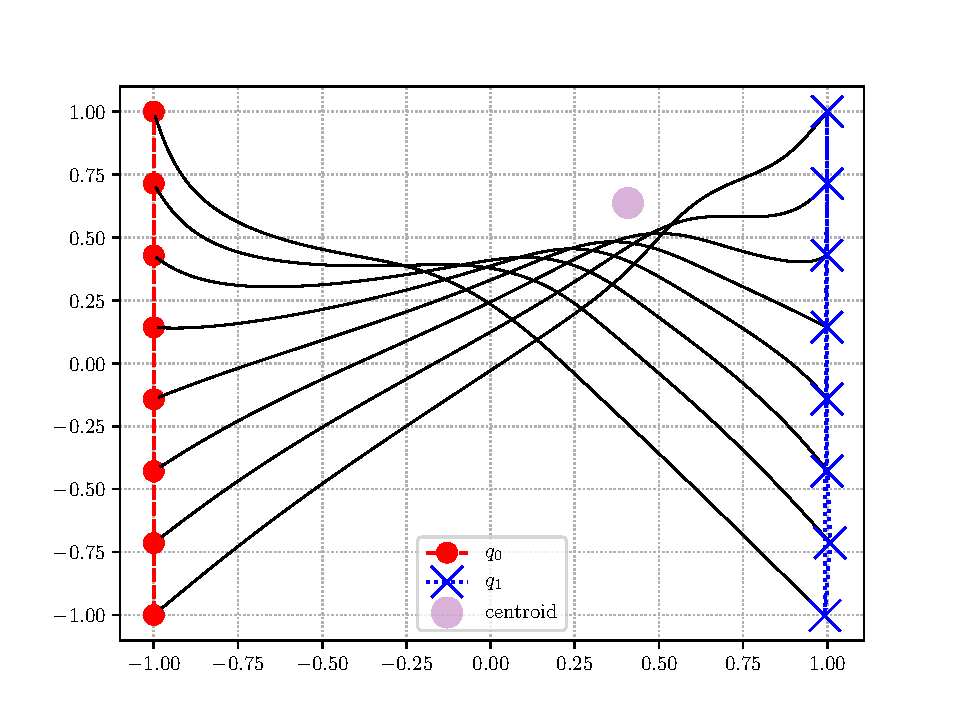
\includegraphics[width=.23\textwidth]{../results/results_criss_cross/sample_4500.pdf}
    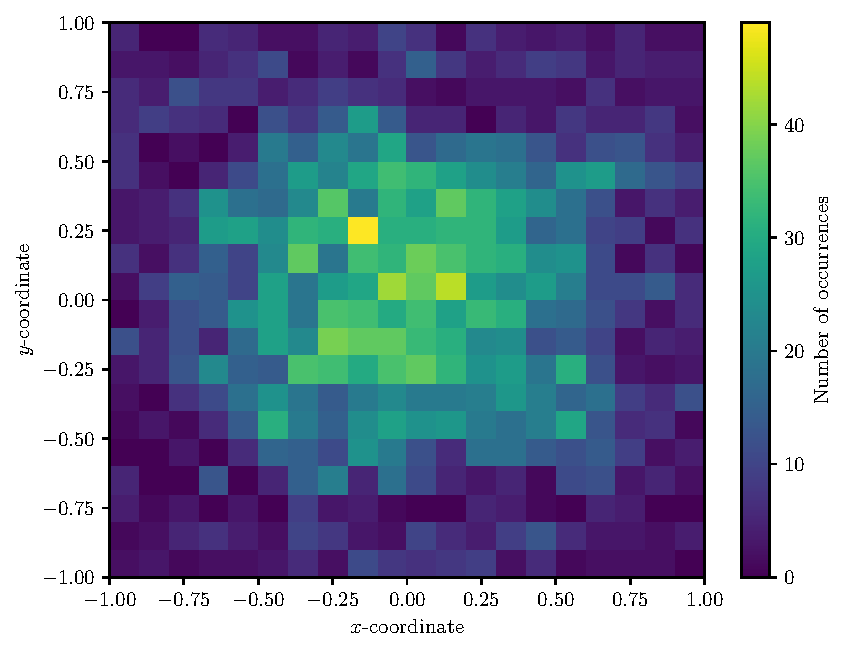
\includegraphics[width=.23\textwidth]{../results/results_criss_cross/centroid_heat.pdf}
    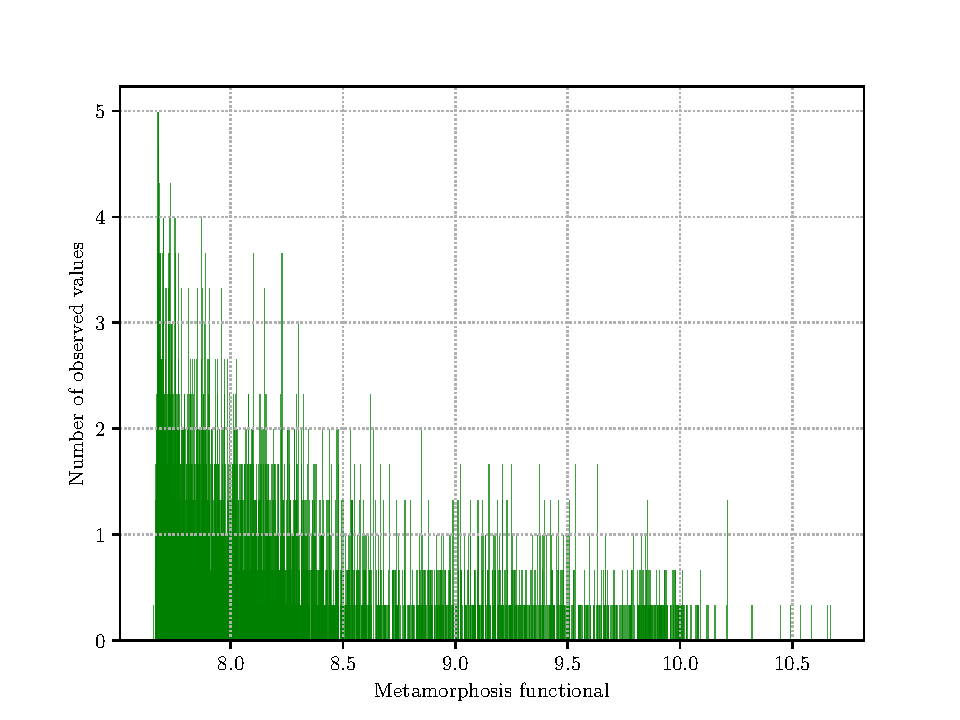
\includegraphics[width=.23\textwidth]{../results/results_criss_cross/functional_histogram.pdf}
    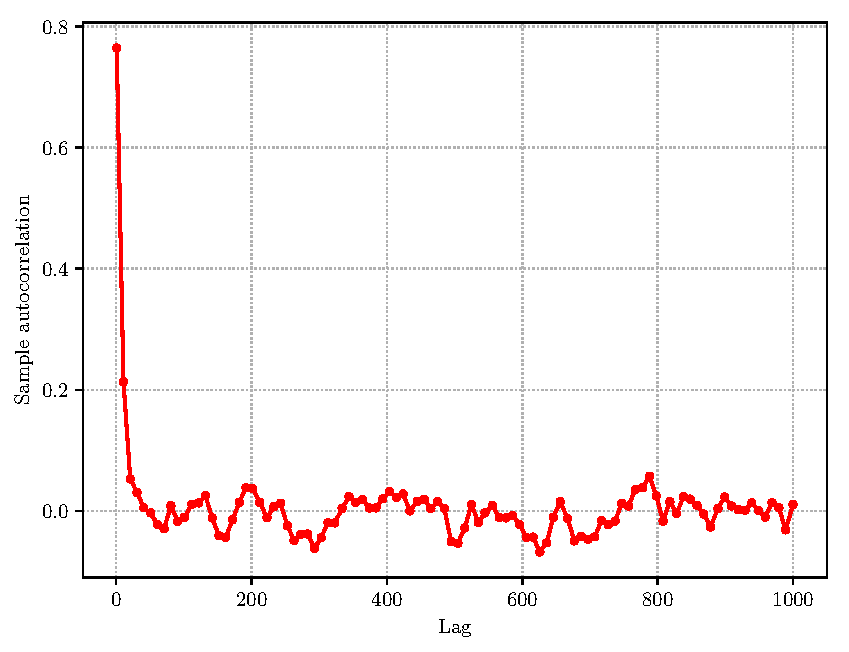
\includegraphics[width=.23\textwidth]{../results/results_criss_cross/autocorrelation.pdf}\\[0.23cm]
    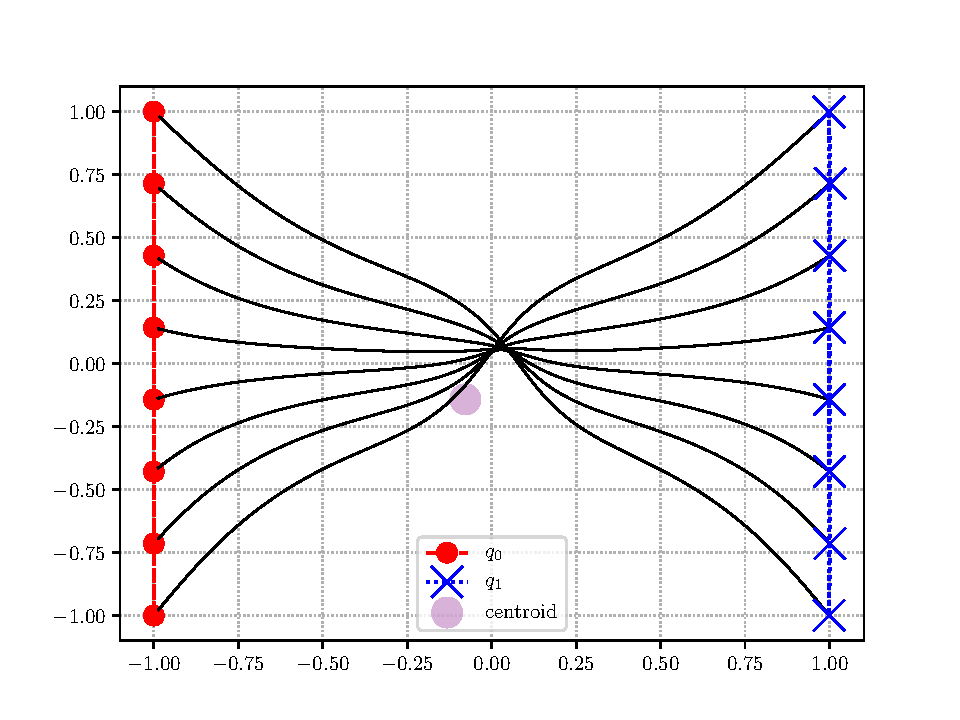
\includegraphics[width=.23\textwidth]{../results/results_criss_cross/MAP_center_0.pdf}
    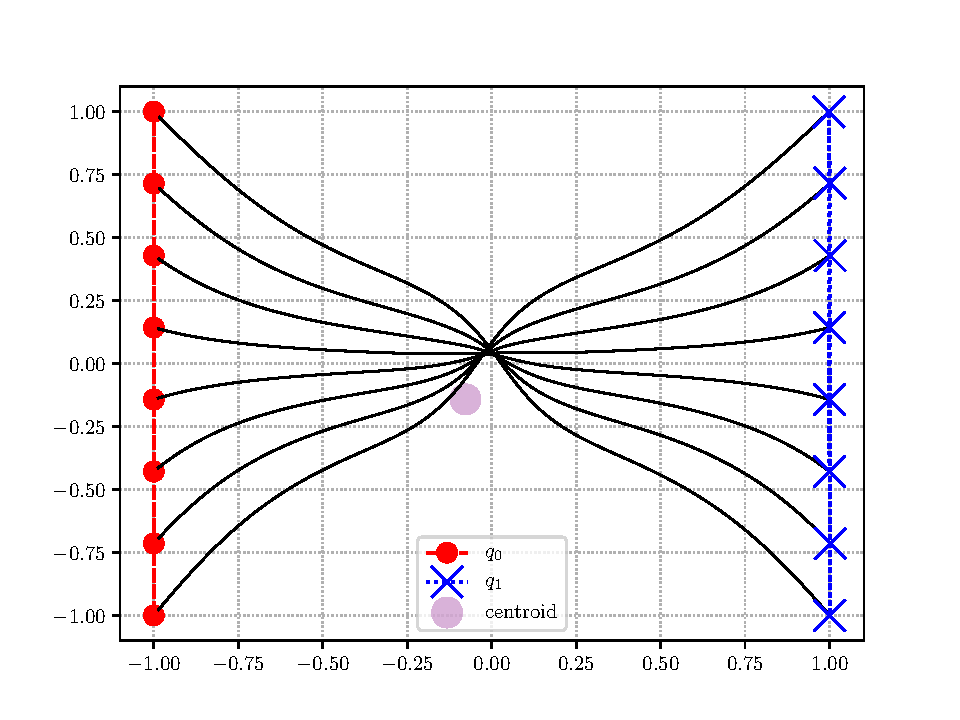
\includegraphics[width=.23\textwidth]{../results/results_criss_cross/MAP_center_1.pdf}
    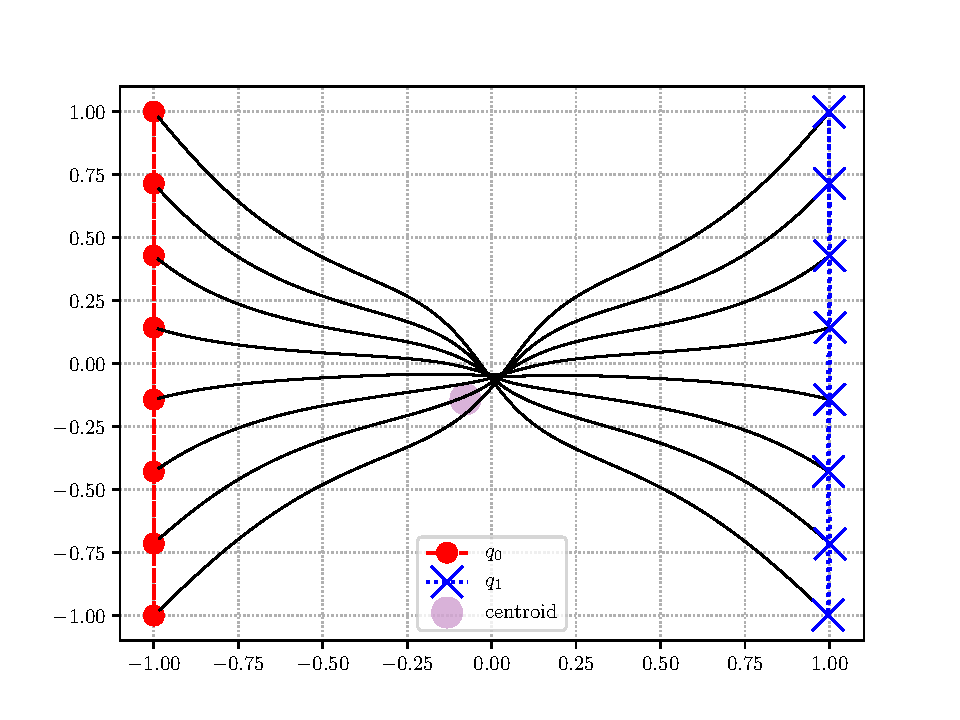
\includegraphics[width=.23\textwidth]{../results/results_criss_cross/MAP_center_2.pdf}
    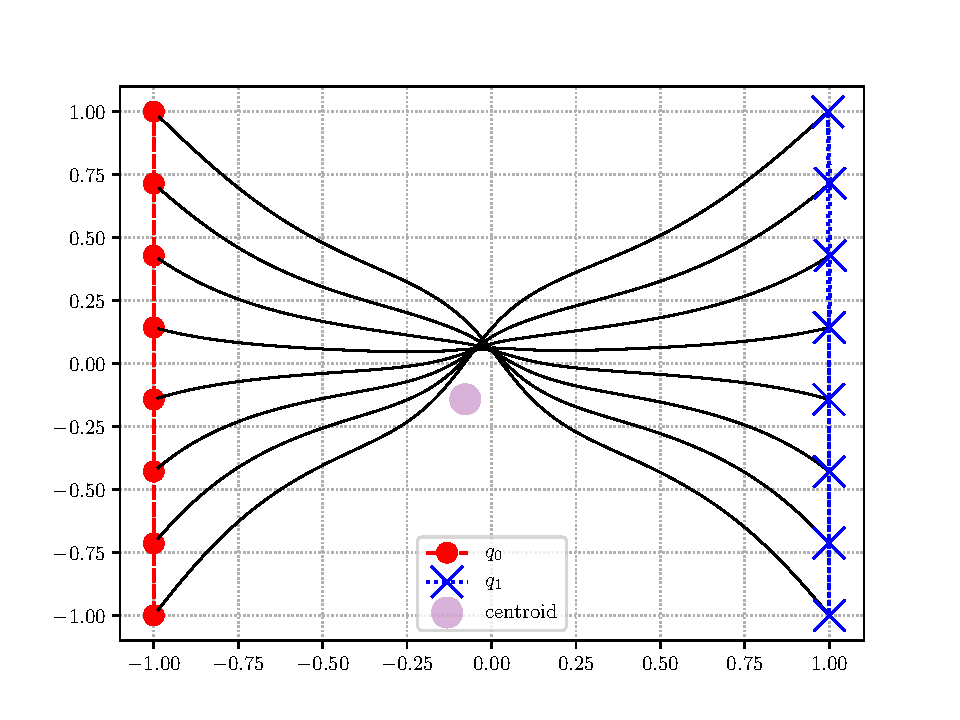
\includegraphics[width=.23\textwidth]{../results/results_criss_cross/MAP_center_3.pdf}
    %\subcaption{.}
    \caption{Selective metamorphosis for the inverted landmarks example The top
    row displays the geodesics corresponding a sample realisation from the
    chain, centroid heat map, functional histogram and
    autocorrelation plot. The bottom row shows the geodesics for four MAP
    estimators. Here the radius is set to $\sigma_\nu = 0.2$, and $0.7$ for the
    velocity kernel and $\beta=0.2$ across $5000$ samples.}
    \label{fig:selective:crisscross}
\end{minipage}
\end{figure}
\begin{figure}
\centering
\begin{minipage}{\textwidth}
  \centering
    \includegraphics[width=.2\textwidth]{example-image-a}
    \includegraphics[width=.2\textwidth]{example-image-a}
    \includegraphics[width=.2\textwidth]{example-image-a}
    \includegraphics[width=.2\textwidth]{example-image-a}\\[0.25cm]
    \includegraphics[width=.2\textwidth]{example-image-a}
    \includegraphics[width=.2\textwidth]{example-image-a}
    \includegraphics[width=.2\textwidth]{example-image-a}
    \includegraphics[width=.2\textwidth]{example-image-a}
    %\subcaption{.}
    \caption{Selective metamorphosis for the pinch example. The top row displays
    the geodesics corresponding a sample realisation from the chain, centroid
    heat map with four MAP estimators, functional histogram and autocorrelation
    plot. The bottom row shows the geodesics for four MAP estimators.}
    \label{fig:selective:pinch}
\end{minipage}
\end{figure}

It is numerically relatively simple to control the behaviour of $\nu$ by simple
scaling or by adding regularisation terms to \eqref{E_sm-def} to e.g. penalise
Fourier modes far away from the support of the images. Here we demonstrate a
simple, proof-of-concept derivative-free method, but depending on the functional
setting investigating a Metropolis-adjusted Langevin algorithms Langevin is also
subject to future treatment.

\section{Outlook}\label{sec:outlook}

We have presented a preliminary approach for selectively allowing photometric
variation in a diffeomorphic image matching. We analysed the selective
metamorphosis problem and the associated geodesic equation and demonstrated a
proof of concept MCMC approach of inferring the $\nu$ control. This generalises
LDDMM and metamorphosis and could provide a first-order exploratory tool for
physicians to see if the development of a biological feature stems from a few
violations of diffeomorphic evolution. This paper paves the way towards
surgically investigating growth phenomena between topologically different images
in certain areas of the target and template. 

We outline the future work necessary to this end. Firstly, we aim to extend the
equations of section \ref{sec:select_mm} to images e.g. using the kernel
framework in \cite{richardson2016metamorphosis} or developing a space-time
method. Further, as outlined in \ref{sec:bayesian} there are many aspects of the
probabilistic framework that needs rigorous treatment. Beyond the references
therein, see also the work in \cite{dashti2013map}. Natural extensions of our
probabilistic ansatz also includes fully treating $\nu$ as a function and
interpreting the resulting inverse problem through the appropriate
measure-theoretical lens. Moreover, adding a time-dependency to $\nu$ is also to
be explored. Determining truncated Fourier modes of $\nu$ could lead to
efficient numerical methods.\\

Finally, it is our hope that we can extend the theory developed here to
encompass classic metamorphosis; that is to say, to develop the necessary theory
in order to place a stochastic model on the state space consisting of velocities
and source functions. Being able to sample random pairs (MCMC) of these would
permit a novel numerical approach to metamorphosis as well as other problems
shape analysis.

\appendix
\iffalse
\section{$z_t$ derivation}\label{app:z_derivation}

We show $z$ satisfies the continuity equation. Using $z_t = \nu(q_t)p_t$:
\begin{align*} 0 & = \dot{\mathbf p}_t + \mdiv(u_t(\mathbf q_t)^T \mathbf p_t) +
\frac12\nabla\nu(q_i) |p_i|^2\\
& = \frac{d}{dt}\frac{\mathbf z_t}{\mathbf \nu(q_t)} + \mdiv(u_t(\mathbf q_t)^T \frac{\mathbf z_t}{\mathbf \nu(q_t)}) 
    +  \frac12\nabla\nu(q_i) |\frac{\mathbf z_t}{\mathbf \nu(q_t)}|^2\\
& = \frac{\dot{\mathbf z_t}}{\nu(q_t)} - \frac{\mathbf z_t \nabla\nu(q_t)\dot{q}_t}{\nu^2(q_t)} + 
\nabla u_t(\mathbf q_t)^T \frac{\mathbf z_t}{\mathbf \nu(q_t)}
- u_t(\mathbf q_t)^T \frac{\mathbf z_t\nabla \nu(q_t)}{\mathbf \nu^2(q_t)}
    + \frac12\nabla\nu(q_i) |\frac{\mathbf z_t}{\mathbf \nu(q_t)}|^2\\
& = \frac{\dot{\mathbf z_t}}{\nu(q_t)} - \frac{\mathbf z_t \nabla\nu(q_t)(u(q_t)+ \mathbf z_t)}{\nu^2(q_t)} + 
\nabla u_t(\mathbf q_t)^T \frac{\mathbf z_t}{\mathbf \nu(q_t)}
- u_t(\mathbf q_t)^T \frac{\mathbf z_t\nabla \nu(q_t)}{\mathbf \nu^2(q_t)}
    + \frac12\nabla\nu(q_i) |\frac{\mathbf z_t}{\mathbf \nu(q_t)}|^2\\
& = \frac{\dot{\mathbf z_t}}{\nu(q_t)} - \frac{\mathbf z_t\nabla \nu(q_t)}{\mathbf \nu^2(q_t)}u_t(\mathbf q_t)
 - \nabla\nu(q_i) |\frac{\mathbf z_t}{\mathbf \nu(q_t)}|^2\\
&+  \nabla u_t(\mathbf q_t)^T \frac{\mathbf z_t}{\mathbf \nu(q_t)}
- u_t(\mathbf q_t)^T \frac{\mathbf z_t\nabla \nu(q_t)}{\mathbf \nu^2(q_t)})
    + \frac12\nabla\nu(q_i) |\frac{\mathbf z_t}{\mathbf \nu(q_t)}|^2\\
& = \frac{\dot{\mathbf z_t}}{\nu(q_t)}
 - \nabla\nu(q_i) |\frac{\mathbf z_t}{\mathbf \nu(q_t)}|^2\\
& + \nabla u_t(\mathbf q_t)^T \frac{\mathbf z_t}{\mathbf \nu(q_t)} + \frac12\nabla\nu(q_i) |\frac{\mathbf z_t}{\mathbf \nu(q_t)}|^2\\
\end{align*}
\fi

\section{Proof of Theorem \ref{sm-eu}}\label{app:proof:sm-eu}
The functional in \eqref{E_sm-def_p} is not convex so we work with a
reformulation to ensure the required lower semi-continuity. Define a
variable $w^i_t = \sqrt{\nu(q_t^i)} p^i_t$ in the problem:

\begin{align}
\inf_{\substack{u \in L^2([0,1],V)\\ q, w\, \in H^1([0,1],\RdM)}}
    & \int_0^1\half\left (h_l(\mathbf q_t,\mathbf p_t)  +\sum_{i=1}^M |w_t^i|^2\right )\diff{t}\\
    & \dot{q_t^i} = u(\mathbf q_t) + \sqrt{\nu(q_t^i)} w^i_t\\
    & \mathbf q_0,\,\mathbf q_1\text{ fixed}
  \label{pbl:reformulation}
\end{align}

We now show existence of a minimiser to this problem. First, note that owing to
the constraint effectively being a boundary value problem, we cannot always find
a $\mathbf q$ for arbitrary pairs of $(u,\,w)$. We define an bounded operator
$(\mathbf q,\, u)\mapsto \frac{\dot{q_t} - u(q_t)}{\sqrt{\nu(q_t^i)}} := w$:
\begin{align*}
\ltwonorm{w}^2 & = \ltwonorm{\frac{\dot{q}_t^i - u(q_t^i)}{\sqrt{\nu(q_t^i)}}}^2\\
& \leq \nuinf^{-1}\Big(\ltwonorm{\dot{q}_t^i}^2 + \ltwonorm{u(q_t)}^2\Big)\\
\end{align*}
which is clearly bounded since $q\in C^1(0,1,H)$ and since by continuity of $u$.
From this we generate a minimising sequence $(q^n, u^n, w^n)$ admissible to
\eqref{pbl:reformulation}.\\

\textbf{$\longrightarrow$ Show weak continuity of the constraint equation for
$q$ (the stuff below)}\\

Passing to subsequences where necessary we can by classic results
\cite{younes2010shapes} extract bounded subsequences converging to weak limits
where necessary to obtain a minimiser. Convexity of $S$ implies the necessary
weak lower semi-continuity concluding the proof.

%\begin{theorem}[Optimality Conditions]
%There exists a unique (? )solution $u, q, z$ to this system.
%This will give more conditions on $\nu$, like $\nu(x) \in C^{1}(\mathbb R^2)$. 
%\end{theorem}

\iffalse
\section{Well-posedness of the equation of motion}
Using the equation for $z$, we can formally write $z_t = z_t \circ \varphi^{-1}$,
which corresponds to writing the initial $z_0(x) = \sum_i z_0^i\delta(x-x_0^i)$, 
and the time dependent solution $z_t(x) = \sum_i z_0^i\delta(x-q_t^i)$ (see 
\cite{holm2009euler}[sec 11.2] for more details). Together with the relations 
\eqref{q_t} and \eqref{z_eta} and $\eta_0 = q_0$ as $\varphi_0 = Id$, we can write
\begin{align*}
  \mathbf q_t &= \varphi_t \eta_t\\
   &= \varphi_t \mathbf q_0 + \varphi_t \eta_t-\varphi_t \eta_0\\
   &= \varphi_t \mathbf q_0 + \varphi_t \int \dot \eta_t dt\\
   &= \varphi_t \mathbf q_0 + \varphi_t \int \varphi_t^{-1} \varphi_t\dot \eta_t dt\\
   &= \varphi_t \mathbf q_0 + \varphi_t \int  \varphi_t^{-1}\mathbf z dt \\
   &= \varphi_t \mathbf q_0 + \varphi_t \int  \varphi_t^{-1}\nu(\mathbf q_t) \mathbf p_t  dt\\
   &= \varphi_t \mathbf q_0 + \varphi_t \int  \varphi_t^{-1}\mathbf z_0\circ \varphi_t^{-1} dt\, , 
\end{align*}
and directly verify that it satisfy the equation of motions by computing
\begin{align*}
  \dot {\mathbf q}_t = \dot \varphi_t \varphi_t^{-1} \varphi \mathbf q_0 + \dot
  \varphi_t \varphi_t^{-1} \varphi_t \eta_t + \varphi_t \dot \eta_t  = u_t(
  \mathbf q_t) + \mathbf z_t\, ,
\end{align*}
using $\dot \varphi_t\varphi_t^{-1} = u_t$. 
This is the integral form of the equation of motion, which is the same equation
as in \cite{holm2009euler}[eqn 19], with the only difference in the term $\nu(q) p_i$ 
in the reconstruction relation. 
{\color{red} Can we simply redo the same proof, but being careful when they need this term, 
and make sure that $\nu(x)<\nu_{max}$ is enough? maybe the derivative needs to be smooth, too. }
\fi

\bibliographystyle{abbrv}
\bibliography{landmarks}
\end{document}
